\section*{Суммирующий счётчик с $K_{\text{СЧ}} = 6$}
\addcontentsline{toc}{section}{К155ИЕ6}

\subsection*{Построение счетчика}
\addcontentsline{toc}{subsection}{Построение счетчика}

Для построение счетчика с коэффициентом пересчета на основе К155ИЕ6 необходимо определить условия сброса.
Поскольку требуется построить коэффициент пересчета 6, то необходимо производить сброс, когда
значение коэфициента равняется $6_{10}=0110_2$. \par

Далее определим управвляющую функцию, которая при выходе счетчика равном 0110 будет передавать логическую 
1 на вход сброса счетчика.

$$
    Y=\overline{X}_0X_1X_2\overline{X}_3
$$

Согласно управляющей функции построим модуль и подклюим его в выходам счетчика. Управляющий сигнал модуля 
подключим к входу сброса через логичское ИЛИ, чтобы сброс происходил либо по входному сигналу сброса, либо при
выходе счетчика 0110.

\begin{figure*}[h!]
    \centering
    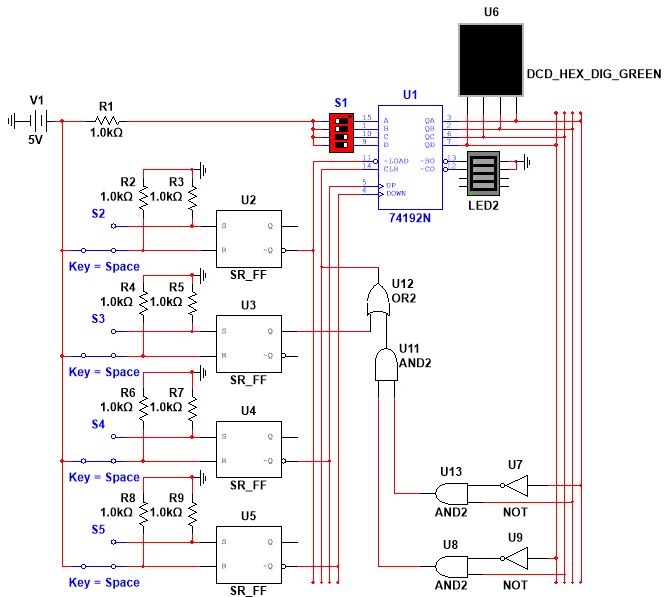
\includegraphics[scale=0.8]{images/image-13.png}
    \captionof{figure}{Суммирующий счетчик с $K_{\text{СЧ}} = 6$}
    \label{image:13}
\end{figure*}

Счетчик был протестирован. Коэффициент пересчета соответвует ожиданию.
